\chapter{Introduction}

Until the release of Dungeon Keeper\footnote{Bullfrog Productions, 1997} most well known fantasy 
video games have allowed the player to play as various heroic characters, raiding dungeons filled
with evil forces in order to acquire treasures and fame.
In Dungeon Keeper, however, we join the opposite faction and try to defend our own dungeon
(along with all the treasures hidden in it) from endless hordes of heroes trying to pillage our domain.
Although we can still play the original Dungeon Keeper today, we cannot change its data or game mechanics
in any easy way so this thesis aims to recreate and modify the original game and extend it to have an easy to 
use programming interface that will allow such modifications.

\section{Dungeon Managment Genre}

Dungeon Keeper was the first game released in the dungeon management~(DM) genre and since our game is going to be based on
Dungeon Keeper, we should design it with the elements of its genre in mind. Since the definition of this genre has to our
knowledge never been formally documented by the creators of Dungeon Keeper, we are going to create a list of basic elements
of the genre based on the gameplay of the original game.

In Dungeon Keeper, the player's main goal is to build and protect his own base, called the dungeon. They do so by commanding
their underlings -- often called minions -- whom they can command to mine gold, which is a resource they use in order to build new rooms
and cast spells (in the game's sequel\footnote{Dungeon Keeper 2, Bullfrog Productions, 1999}, mana was added into the game
as a secondary resource used for spell casting), which could be researched as the game progressed. They would then use creatures
spawned in their buildings as well as their own magic powers to fight intruders in order to protect their dungeon. 
From this brief gameplay summary, we can create list of the most basic design elements, which can be found in dungeon management games:

\begin{enumerate}[label=\textbf{(E\arabic*)}]
    \item Resource management
    \item Dungeon building
    \item Minion commanding
    \item Combat
    \item Player participation in combat
    \item Research
\end{enumerate}

Now that we have created a list of the genre's basic design elements, let us have a look at how they were implemented in games from the
Dungeon Keeper series.

\subsubsection{Resource management}

In the original Dungeon Keeper, the player used gold as their primary resource. They would have it mined by their minions and use
it to build new rooms and cast spells. While having a single resource for everything may bring simplicity to the game, it also means
that once the player runs out of gold, they will not be able to directly participate in combat due to their inability to cast spells.
It is for this reason that we are going to use the resource model of Dungeon Keeper 2 and have a separate resource -- mana -- that
will be used to cast spells.


\subsubsection{Dungeon building}

The term dungeon building in Dungeon Keeper refers to tearing down walls in order to create new rooms which the player's minions 
then claim and the player can place new buildings in. These buildings can then act as gold storage, spawn new creatures or be used
as traps that negatively affect attacking enemies. Since this is a central theme in Dungeon Keeper (and dungeon management games
in general), we should try to implement our building model to resemble this one.

\subsubsection{Minion commanding}

The term minion commanding stands for giving your minion tasks such as to move somewhere, attack an enemy or tear down a wall. In
Dungeon Keeper, most of these commands were implemented as spells -- although mining was done by simply selecting blocks, which
could unfortunately cause minions to destroy walls the player accidentally selected. To provide a unified interface to minion tasks
and to avoid the accidental block destruction, all commands the player can give should be in our game implemented as spells.


\subsubsection{Combat}

In Dungeon Keeper, the player's dungeon is under frequent attacks by enemy heroes. These enemies attack the dungeon 
in groups with a delay between each two attacks, in a similar way to tower defense games (e.g. Orcs must die!~\cite{OMD} 
and Dungeon Defenders~\cite{DungeonDefenders}), where they are often referred to as \emph{waves}. Each wave of enemies
can consist of different types of heroes and the delay between waves can differ, too. Since the players of the original
Dungeon Keeper are already familiar with this wave system and it may also satisfy the players of tower defense games, we will be
implementing it in our game.

\subsubsection{Player participation in combat}

During the fights with enemy heroes, the player in Dungeon Keeper can cast various spells to affect the outcome of the battle.
These spells can have various forms from spawning creatures, damaging enemies and healing minions to destroying walls and throwing
meteors. If we want to create a similar spell system, we need to support these different types of spells, e.g. targeted spells that
affect a single entity, positional spells that can summon a creature or global spells, that simply have an effect on the game once
they are cast.

\subsubsection{Research}

In the original Dungeon Keeper, researching new spells and buildings was done through a special type of room, called the library,
which can be seen in Figure~\ref{dk-lib}. There,
various minions could study and achieve new advancements for the player after a certain amount of research points -- which was different
for different spells and buildings -- was gathered. But this design decision brought a negative element into the game, because once the
library was destroyed by the heroes, the player was unable to perform additional research and could not even use the ability to cast
some spells. This is why we are going to use a different approach, called the research tree (or sometimes the technology tree), first used
in the turn-based strategy game called Sid Meyer's Civilization\footnote{Developed by MPS Labs, 1991}, as pointed out by Tuur Ghys in his
article about technology trees~\cite{ResearchTrees}. This approach 
separates the research from the events happening in the game and allows the player to research new advancements for a resource (e.g. gold),
with each new technology, building, creature or spell being able to have prerequisites.

\begin{figure}[H]
    \centering
    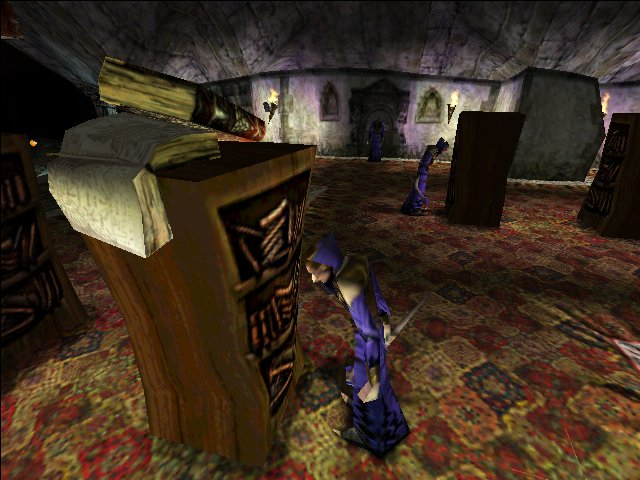
\includegraphics[width=10cm]{../img/library.jpg}
    \caption{Warlocks researching in the library.
             \\Source: \href{http://vignette2.wikia.nocookie.net/dungeonkeeper/images/9/98/Library.jpg/revision/latest?cb=20120808211437}{http://dungeonkeeper.wikia.com}}
    \label{dk-lib}
\end{figure}

\section{Modifiability in Games}

One of our basic goals is for our game to be modifiable, which means to provide tools -- often called \emph{modding tools} -- to our players
that will allow them to create modifications -- often called \emph{mods} -- that other players can install and which can change or
add elements to the game.

This can increase the replay value of the game as after finishing it, more missions, characters, game mechanics, abilities, items
or even game modes can be easily downloaded and installed from internet. Since we want our game to be modifiable as much as
possible, an important topic we need to decide on is which parts of the game we will allow the players to modify. 
An example of an easily modifiable game is Minecraft~\cite{Minecraft}, a 3D sandbox game 
in which the player has to survive in a procedurally generated world. Let us now examine the basic concepts of the game before
we investigate concrete examples of mods and how they changed the game in the following sub chapters. 
As a reference, a screenshot of Minecraft can be seen in Figure~\ref{minecraft}. 

\begin{figure}[H]
    \centering
    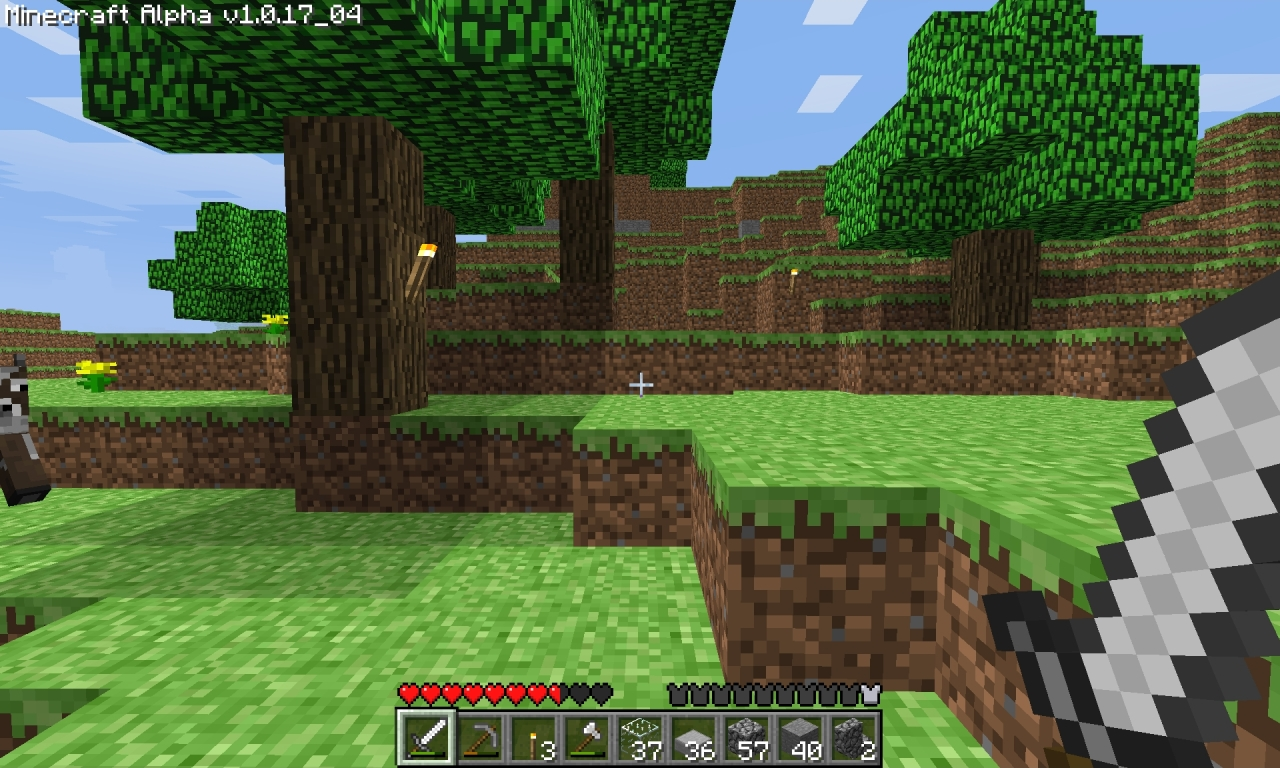
\includegraphics[width=10cm]{../img/minecraft.jpg}
    \caption{Screenshot of Minecraft.
             \\Source: \href{http://i.neoseeker.com/p/Games/PC/Simulation/City/minecraft\_image\_zx2AU2n6bZho0lz.jpg}{http://www.neoseeker.com}}
    \label{minecraft}
\end{figure}

In the screenshot we can see a player standing in the game's world, equipped with an iron sword that can be used for self-defense when the
player is attacked by enemies or to kill animals in order to acquire food required to restore one's health, standing next to a hill and
a couple of trees. Everything in the game is made of \emph{blocks}, which are items that can be placed in the world and
-- with some exceptions\footnote{E.g. the bedrock block, which covers
the bottom layer of the world and prevents the player from falling outside of the world's boundaries} -- destroyed so that the player
can place them in their inventory. They can either be used for building or they can be interactive, which the player can right click on
to trigger their functionality -- e.g. show a special window or change their state. An example of an interactive block is the chest block,
which provides additional item storage when the player interacts with it.

In the bottom part of the screen we can see the hotbar, which the player can use to store commonly used items 
like tools -- e.g. a pickaxe, which is used to mine blocks,
or an axe, which is used to cut down trees and allows the player to harvest wood -- and blocks, which can be used for building or
crafting.

Crafting is an important part of Minecraft. It allows the player to create tools and complex blocks by combining one or more crafting
ingredients -- e.g. wood, stone, iron or food. The crafting system in the game is based on different crafting recipes, which restrict
what items and in what composition on the game's crafting window -- either a two by two window in the player's inventory screen
or three by three window shown when the player uses a special interactive block called the crafting bench.

\begin{figure}[H]
    \centering
    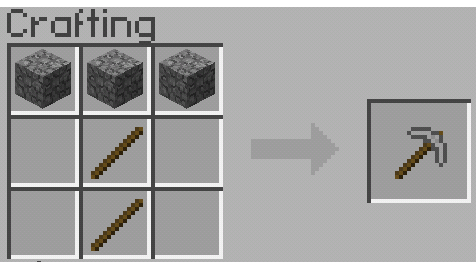
\includegraphics[width=10cm]{../img/MCCrafting.png}
    \caption{An example of a crafting recipe in Minecraft, the player can create a stone pickaxe by combining two wooden sticks
             with three stone blocks.
             \\Source: \href{http://thecoolestminecrafters.weebly.com/uploads/2/6/3/1/26317386/912472788.png}{http://thecoolestminecrafters.weebly.com}}
    \label{minecraft-crafting}
\end{figure}

Figure~\ref{minecraft-crafting} shows an example of such crafting recipe, specifically the pickaxe crafting
recipe. The existence of this recipe in the crafting system means that if a player interacts with the crafting bench and places
two wooden sticks and three stone blocks -- although different resources like iron or gold bars can be used for a different type
of pickaxe -- in the layout shown in the picture, the crafting bench will produce a stone pickaxe in exchange for the resources.

\subsection{Mod examples}

There are thousands of different minecraft mods -- for example, the mod repository at Curse.com~\cite{CurseMods} contains
over 4 thousand mods and the one at PlanetMinecraft.com~\cite{PlanetMinecraftMods} contains even over 7 thousand different mods.
To find the right moddable features of our game, we will now look at some examples of these mods and see how they change Minecraft.

\subsubsection{Industrial Craft 2}

The first example is called Industrial Craft~2~\cite{IndustrialCraft}. This mod adds new blocks and tools as well as a new game mechanic
-- the concept of electricity -- to the game. The items added by the mod range from simple ones like new types of armor or
new tools to complex blocks like various electricity generators and automatized machines.

An example of such machine is the electric furnace. In the game without mods, the player gets iron and other metals in the form
of a raw ore when they mine a block containing the metal. To use the metal in a crafting recipe, the players needs to smelt the ore
into a bar using the furnace, which can be powered by wood or coal. The electric furnace uses electricity for power and can be
powered by an electricity generator -- e.g. a solar panel -- which removes the necessity to repeatedly place wood or coal in
the machine.

\begin{figure}[H]
    \centering
    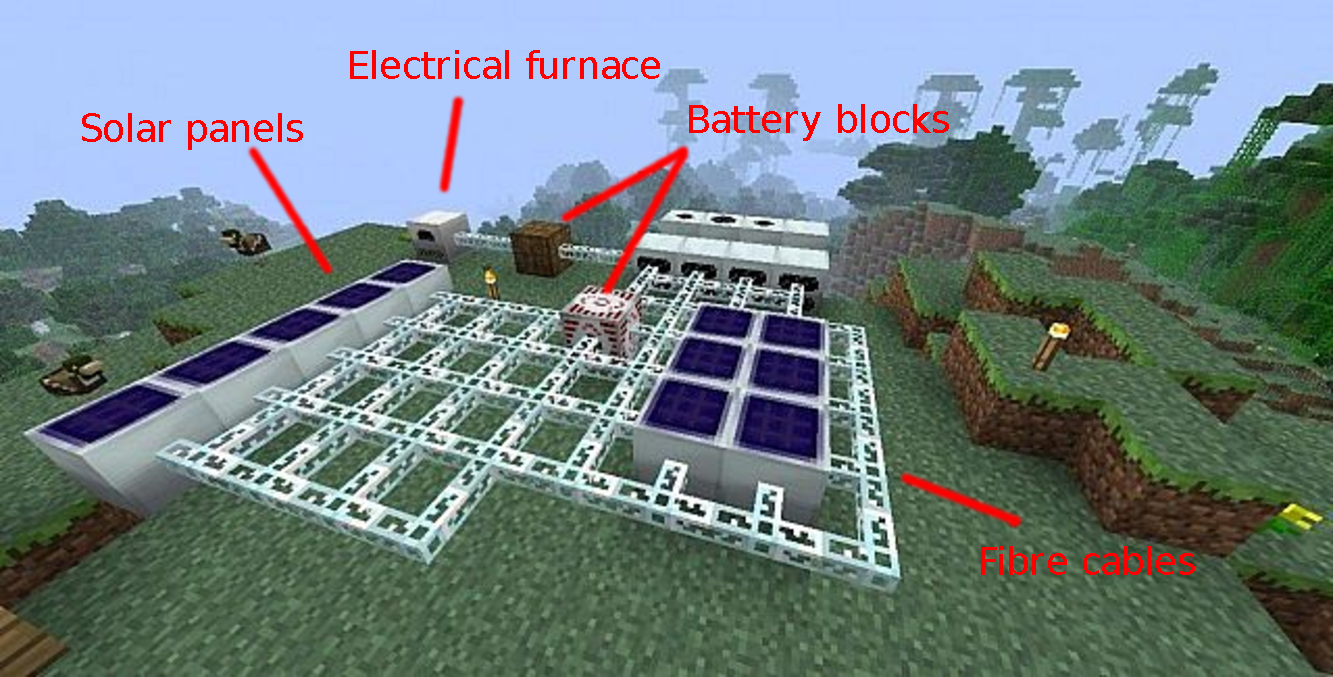
\includegraphics[width=10cm]{../img/ic-solar.pdf}
    \caption{A simple setup powering multiple machines including an electrical furnace using solar panels.
             \\Source: \href{http://static.planetminecraft.com/files/resource\_media/screenshot/1246/javaw-2012-11-12-20-51-09-46\_4122139.jpg}{http://www.planetminecraft.com}}
    \label{ic-solar}
\end{figure}

In Figure~\ref{ic-solar}, we can see a simple setup in which a couple of solar panels are connected to an electric furnace and other
machines via glass fiber cables. We can also see another interactive block added by the mod -- the battery block. The battery block
stores electricity up to a certain capacity and continues powering the machines even when its electricity input stops, which in the
case of solar panels can happen during the night.

Using these machines, the game can be changed from its rather primitive setting -- in which the player mines resources with simple
tools and builds simple houses -- to a modern setting with automated mining and resource processing machines. If we want to allow
the players of our game to create similar modifications, they should be able to change existing and create new buildings -- our equivalent of 
Minecraft's blocks -- which includes changing their appearance, the way they function -- e.g. what type of minions they spawn -- and
how they interact with enemies.

\subsubsection{Computer Craft}

Another mod, called ComputerCraft~\cite{ComputerCraft}, added fully functional computers into the game. 
These computers can be used to create password protected
doors, write programs and games in the Lua programming language~\cite{Lua} or even connect to internet services such 
as IRC\footnote{Internet Relay Chat, an open communication 
protocol.} or telnet\footnote{A client-server protocol, that allows bidirectional text-oriented communication through a terminal.}.

\begin{figure}[H]
    \centering
    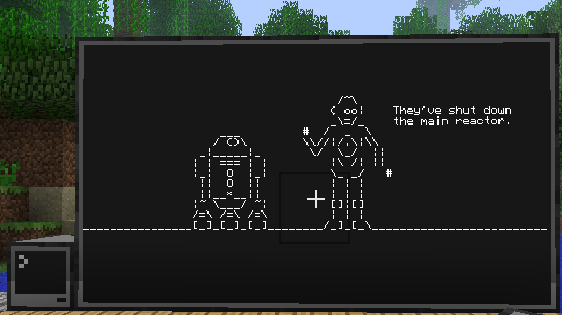
\includegraphics[width=10cm]{../img/ComputerCraft2.png}
    \caption{A computer in Minecraft playing the ASCII version of the movie Star Wars: A New Hope.
             \\Source: \href{http://minecraft-modding.de/wp-content/uploads/2015/06/ComputerCraft2.png}{http://www.minecraft-modding.de}}
    \label{computer-craft}
\end{figure}

An example of such computer in minecraft can be seen in Figure~\ref{computer-craft}. There, a player has connected a computer to a screen
and used the computer to connect to a server via telnet. The server then sent back messages that, when displayed sequentially, played
the first Star Wars movie.

\begin{figure}[H]
    \centering
    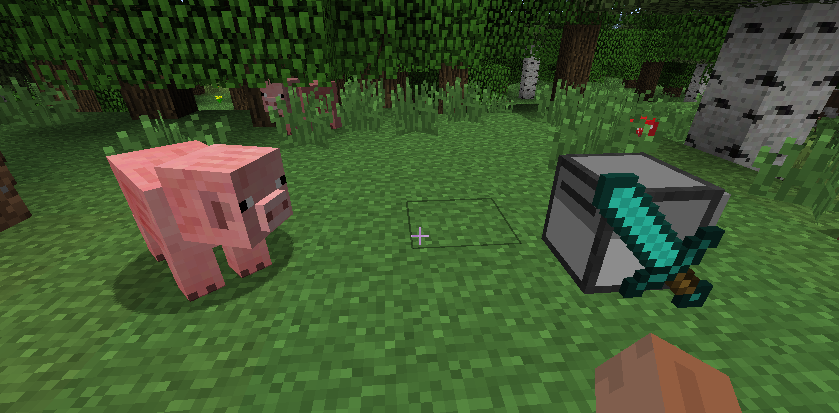
\includegraphics[width=10cm]{../img/CC-turtle.png}
    \caption{A turtle equipped with a diamond sword about to attack a pig.
             \\Source: \href{http://computercraft.info/wp-content/uploads/2012/07/piggy.png}{http://www.computercraft.info}}
    \label{cc-turtle}
\end{figure}

This mod also added robots into the game. These robots -- called \emph{turtles}, inspired by the Logo programming language -- 
could be programmed using Lua scripts to automate 
various tasks. The task a turtle fulfills is determined by the tools it is equipped it. If, for example, the player gives it a pickaxe, 
the turtle will then be able to mine blocks and being equipped with an axe will allow it to chop down trees. 
In Figure~\ref{cc-turtle}, we
can see another type of a turtle, this time equipped with a sword. The mod provides the player with an API in which they can write
instructions for the turtle. If, for example, these instructions were in this case 'walk three times forward and attack' 
-- written in Lua -- the turtle would walk forward and killed the pig standing in front of it.

We have already decided to allow our players to modify the buildings in our game, based on the machines in Industrial Craft~2. 
From Computer Craft, we are going to take the concept of minion and enemy modification. This means that the players
of our game should be able to change the attributes of both minions and entities in the game, including attributes such as health and
damage, abilities, spells and most importantly, their overall behavior (i.e. their artificial intelligence).

\subsubsection{Team Fortress 2 Map}

Aside from adding items and creatures, entire new games can be created within a modifiable game.
One of the interactive blocks in Minecraft is the command block,
which can execute commands in the game's developer console -- e.g. teleport the player to a certain position or give him items --
when the player right clicks it.

One of the players of the game, called Seth Bling, used this block to create a map which alters the way the game is 
played~\cite{FutureOfMinecraft}. For example, even though the 
unmodded game has no concept of character classes, he used the command block to equip the player that clicked on it with a special
set of tools and weapons, using the command to add items. Multiple of these blocks -- each with a different set of items -- 
allowed him to emulate classes in the game. Then, using the same block with different setting, he created control points which
the players could stand on to capture them. Using these control points he was then able to alter the game's winning condition, which
was originally to kill a specific enemy, to a requirement team of players having all control points in the world under their control.
Once all control blocks were controlled by the same team, another command -- requesting the game's end -- would be executed.

The result of these modifications was the change of Minecraft to look and play like another game, called 
Team Fortress~2~\cite{TF2}. Team Fortress~2 is a 3D first person shooter, in which two player teams fight against each other in various
game modes, e.g. the aforementioned point control. Each player in the game can choose from a wide selection of character classes, 
each with its own attributes and weapons.

Unlike Industrial Craft~2 and Computer Craft, which only added new items and non-player characters into the game, this map mainly altered
two aspects of the game. Firstly, it changed the way the player plays the game by limiting them to a specific number of different
classes they can play, bringing diversity to the game's online play. Secondly, it changed the way the game ends, i.e. under what condition
the player wins or loses.

From this map, we are going to take the ability to modify these exact two aspects. While the change of the game's end condition can be done
similarly to the way it was done in this game -- i.e. executing a custom command to win or lose the game, the change of the play style can
not be done by item restriction because in our game the player has no items. The way that, in our game, the player interacts with the world
is through their spells -- which include entity commanding. This means that alongside building, minion, enemy and end condition modification,
our players should be able to change their spells and create new ones. These changes should be able to affect the gameplay, so they should
range from simple damage and range modification to complete changes of the effects these spells have on the world.

One important note is that this change of gameplay was not done by creating a mod but was created as a map for the game, which the players
could download from internet and then simply load in the game without any installation.
This way of distribution of changes to the game, alongside modding, creates
another way for the players of a game to create and share modifications of the game. Since we want our game to be modifiable, we should
implement a way for our players to create similarly game changing maps in our game, i.e. we should store our levels
in a format that will allow later modifications, including actual changes to the game's elements.

\subsubsection{Conclusion}

In conclusion, we can see that the ability to modify a game can help said game to grow even when its development has stopped
or is focused in different areas (e.g. security, stability). Since we want to give this ability to the players of
our game, our modding tools should allow them to change some of its data, including but not limited to:

\begin{itemize}
    \item Minions and enemies -- e.g. changing attributes such as health and damage, displayed models, behavior and spells they
        cast.
    \item Buildings -- e.g. changing their size, models, types of creatures that they spawn and, in the case of traps, their interaction with
        enemies.
    \item Spells -- fully changing the effect of a spell, e.g. from simple damage dealing to spawning a meteor shower.
    \item Goals of the game -- changing requirements for winning the game or the reasons for a loss.
\end{itemize}

Besides changing data of entities -- e.g. creatures, buildings or spells -- the players should also be able to create new types of these
entities.

The game on its own, like Minecraft, should also be fully featured, offering enough of these entities
on its own so the players do not need mods to actually play the game. Additionally, since our game, like Dungeon Keeper,
will have scripted waves of enemies attacking the player's dungeon, the also should allow our players to alter the wave 
composition -- that is, which types of enemies compose the different groups attacking the player's dungeon --  and delays between
the waves. Last, but not least, we must not forget that players do not necessarily have to be (and often are not)
programmers, so our game should provide an easy way to install these modifications.

\section{Competitiveness of the game}

We have now investigated the main design elements of Dungeon Keeper and how we are going 
to implement them in our game. The last thing we have to realize is that since we are trying to satisfy the players of the original
game, the resulting product of our work should be a full game and not just a prototype. This means that the game should offer full 
singleplayer experience, with relatively intelligent enemies and the ability to not only win the game, but to also lose. 
Also, for the game to be competetive with other titles,
it should be performant, achieving at least the minimum acceptable framerate, defined as 25-30 frames per second by 
Shiratuddin, Kitchens and Fletcher~\cite{AcceptableFPS}, on both new and older hardware.

\section{Thesis Goals}

The main goal of this thesis is to design and implement a modifiable 3D dungeon management game using the design elements \textbf{(E1)}~--~\textbf{(E6)}.

In addition to the main goal, the game should complete the following list of goals:

\begin{enumerate}[label=\textbf{(G\arabic*)}]
    \item The game has to be a full competetive product, not a prototype.
        \begin{enumerate}[label=\textbf{(G1.\arabic*)}]
            \item It has to be performant, achieving high framerate even on low end computers.
            \item It has to offer full single player experience, including enemies with scripted behavior and a chance to both win and lose.
            \item It has to contain a variety of entities, spells and buildings even without mods.
        \end{enumerate}
    \item The game has to be highly modifiable, providing an easy to use modding interface for players.
        \begin{enumerate}[label=\textbf{(G2.\arabic*)}]
            \item The mod creators must be able to create new entities (including their behavior), spells and buildings and to 
                change characteristics of already predefined entities, spells and buildings including, but not limited to
                health, damage, model, behavior and abilities of an entity, effect of a spell  and which kind of minion does a building spawn.
            \item They must also be able to alter the game progression by defining enemies that spawn and delays between them.
            \item The game should also support the creation of custom levels.
        \end{enumerate}
    \item The mods for the game have to be easily installable even by players without any programming knowledge. 
\end{enumerate}
